%% LaTeX.tex
%% Example for the proceedings of the 19th Brazilian Congress of Thermal Sciences and Engineering
%% ENCIT 20222
%% November, 6-10, 2022 (Online)
%% Based on the template of the proceedings of ENCIT2020

\documentclass[10pt,fleqn,a4paper,twoside]{article}
\usepackage{abcm}
\def\shortauthor{F. Author, S. Author and T. Author (update this heading accordingly)}
\def\shorttitle{Paper Short Title (First Letters Uppercase, make sure it fits in one line)}

\begin{document}
\fphead
\hspace*{-2.5mm}\begin{tabular}{||p{\textwidth}}
\begin{center}
\vspace{-4mm}
\title{Enhancing Experimental and Numerical Data Validation through Acoustic
Noise Signal Demodulation for Estimating Drone Propeller Rotational Speed} %(XXXX is the manuscript number. It will be available after the extended abstract submission and must be placed for the final paper submission.)
\end{center}
\authors{Gabriel Costa da Silva} \\
\authors{Mateus Grassano Lattari} \\
\institution{Federal Univerisity of Santa Catarina, UFSC} \\
\institution{gabriel.silva@polo.ufsc.br} \\
\institution{mateus.grassano@polo.ufsc.br} \\
\\
\authors{Lucas Bonomo Araújo} \\
\authors{Julio Codioli} \\ 
\authors{Racquel Knust Domingues} \\
\authors{Augusto Barth Beck} \\ 
\institution{Federal Univerisity of Santa Catarina, UFSC} \\ %(If all authors are from the same institution, the "Institution and address" must be placed only once.)
\institution{lucas.bonomo@lva.ufsc.br} \\
\institution{julio.cordioli@ufsc.br} \\
\institution{racquel.knust@lva.ufsc.br} \\
\institution{augusto.barth.beck@gmail.com} \\
\\
\abstract{\textbf{Abstract.} This study addresses a novel approach for estimating the rotational speed of
small-scale propellers, typically found in drones, through the analysis of their
acoustic noise signal. Accurately determining the instantaneous rotational speed
of propellers in anechoic wind-tunnels poses significant challenges due to
inherent experimental rotational speed fluctuations. These fluctuations can
distort harmonic peaks levels, or deteriorate the process of applying comparable
techniques when validating constant rotational speed numerical simulations with
experimental data. This can be overcome by the knowledge of the propeller
instantaneous rotational speed, allowing the signal to be resampled, correcting
it to a constant rotational speed. Measured tachometer data is often not
available nor reliable, as the use of external devices is not always feasible
due to space constraints, costs, and sensitivity to adverse environmental
conditions. An alternative approach is to directly estimate the propeller
rotational speed from the measured acoustic signal, which is the focus of this
study. The proposed methodology is based on the signal demodulation, which is a
tacholess method that calculates the Hilbert Transform of the acoustic signal to
obtain the frequency and phase related to the shaft rotation. To evaluate the
technique, a synthetic propeller noise data are generated with a previous
established rotational speed fluctuation, allowing a characteristic error for the
algorithm predicted instantaneous rotation to be obtained. Secondly, the process
is repeated for a real propeller noise signal, and the results are compared with
the actual rotational speed measurement obtained with the tachometer. Finally,
the obtained instantaneous rotation is employed to resample the experimental
signal, allowing it to be suitable for validating numerical simulated signals.
The spectra obtained from both signals are then compared, and the signal
components are evaluated using a Time Synchronous Averaging (TSA) analysis.
Preliminary results indicate the consistency and feasibility of the technique.}\\
\\
\keywords{\textbf{Keywords:} Propeller noise, frequency estimation,signal processing, aerodynamic noise.}\\
\end{tabular}

\section{INTRODUCTION}
In the ever-evolving realm of drone technology, the precise estimation of propeller rotational speed stands as a pivotal challenge. The need of knowing this information provides further analysis, such as dynamic control, precise noise sources identifications with decomposition techniques and failure prediction.

Upon scrutinizing the acoustic traits of noise produced by fully electric propulsion systems, it becomes apparent that the primary sources are the interactions between the blades and the airflow, encompassing turbulence and vortical effects. The dominant aspect of the noise spectrum comprises the tonal rendition, characterized by multiples of the blade-pass frequency (BPF), signifying a periodic signal. In contrast, the broadband feature, originating from the blade interactions, disperses energy throughout all frequency bands, exhibiting inherent stochasticity. In order to better analyze the noise sources, the features must be separated, which can express plenty dificulties, upon rotational speed fluctuations.

In this context, the Time Synchronous Averaging Method (TSA) \citep{MCFADDEN1987173} finds extensive application in rotors operating at constant rotational speeds, owing to its straightforward implementation and effectiveness in isolating peaks. The method operates by averaging segments of acoustic data corresponding to a single rotation length in the time domain. However, its efficacy diminishes when applied to systems with varying speeds, as the irregular periodicity of segments undermines its performance. \cite{SHARMA2016560} proposed a tonal and broadband components TSA-based decomposition in order to calculate fault indicators in gears, which considerates the rotational frequency fluctuation, therefore, this technique takes in account the tachometer signal, using n pulses per revolution. With this device it is possible to track the angular position of any shaft. 

Small-scale propellers, typically found in drones, necessitate accurate measurement techniques amidst the backdrop of inherent experimental fluctuations. Traditional methods, reliant on tachometer data, often falter due to practical constraints and environmental sensitivities, prompting a quest for alternative methodologies. \cite{article} presents a complete analysis on various methods that discart the need of a tacho signal.

\cite{Urbanek2011ComparisonOA} investigate three major instantaneous frequency estimation techiniques without any phase markers use in wind turbines speed tracking application. The spectrogram-based method proceeds with a maxima tracking due to the fact the peaks with the highest energy on the spectrogram should correspond to the value of the instantaneous frequency at each moment in time.

In another approach,\cite{BONNARDOT2005766} proposed a tacholess technique of estimating the instantaneous rotation of a shaft with limited frequency fluctuations. The method is based on the phase demodulation and utilizes the Hilbert Transform, a matematical instrument to obtain the imaginary part of the analytic signal, which corresponds to the phase of the signal. The main achievement of this technique is that extincts the need of a tachometer, the instant rotation can calculated based on the shaft vibration data. This work analyses the merits and the feasibility of this method.

This work is organized as follows: Section 2 presents the methodology of the phase demodulation technique, describing in details the physics behind the numerical calculation. Section 3 describes some setups of both numerical and experimental data and Section 4 compares the results with the tachometer real information, as well as evaluates the components of the resampled signal with Time Synchronous Averaging (TSA) techiniques. Finally, Section 5 concludes the consistency of the demodulation method.

\section{METHODOLOGY}
Section 1 introduces the importance of the study and begins with a literature review on the current advances in the field. This part of the study is aimed at presenting in details the methodology to be followed in order to perform the instantaneous frequency profile caracterization of a propeller.

First, a widely used mathematical tool in the field of signal analysis is presented. 

\subsection{The Hilbert Transform}

Consider a system with an input $x(t)$ and a filter $h(t) = \frac{1}{\pi t}$. The output of the system is given by:
\begin{equation}
    y(t) = \hat{x}(t) =  h(t) * x(t) = \frac{1}{\pi t} * x(t)
    \label{eq1}
\end{equation}

This convolution operation is called a Hilbert Transform \citep{shin}. Note that $h(t)$ is a non-causal filter with a singularity at $t=0$. The Hilbert transform is often referred to as a 90º phase shifter. For example, the Hilbert transform of $cos(\omega_{0} t)$ is $sin(\omega_{0} t)$, and that of $sin(\omega_{0} t)$ is $-cos(\omega_{0} t)$.

The significance of the Hilbert transform is that it is used to form the so called "analytic signal" or "pre-envelope signal". An analytic signal is a complex time signal whose real part is the original signal $x(t)$ and where imaginary part is the Hilbert transform of $x(t)$, i.e. $\hat{x}(t)$. Thus, the analytic signal $a_{x} (t)$ is defined as:

\begin{equation}
    a_{x} (t) = x(t) + i\hat{x}(t) = A_{x}(t)e^{i\phi_{x}(t)}
    \label{eq2}
\end{equation}
Where $A_{x}(t) = \sqrt{x^2 (t)+ \hat{x}^2 (t)}$ is the instantaneous amplitude, and $\phi_{x} = tan^{-1}(\hat{x}(t)/x(t))$ is the instantaneous phase.

\subsection{The Demodulation Method}
The primary method used for determining the instantaneous frequencies of a two-bladed propeller is the Demodulation Method \citep{BONNARDOT2005766}, a robust and effective procedure that allows for a detailed and precise analysis of dynamic variations over time.

The technique consists of five main steps, each with its own peculiarities and conditions for optimal performance. This will be discussed in detail in Section 5, where the results will be presented.

Firtly, a characteristic harmonic of the signal is selected, with this study focusing on the first Blade Pass Frequency (BPF), which represents the harmonic with the highest energy. Subsequently, through a detailed visual analysis of the spectrum, a band-pass filter is applied to precisely isolate the region corresponding to the shaft rotation harmonic, along with its controlled frequency variations. This approach ensures a focused and accurate examination of the relevant dynamic behaviors. Fig. 1 demonstrated the frequency band selection for the filtering.
\begin{figure}[h]
\centering
\begin{subfigure}{.5\textwidth}
    \label{fig1a}
    \centering
    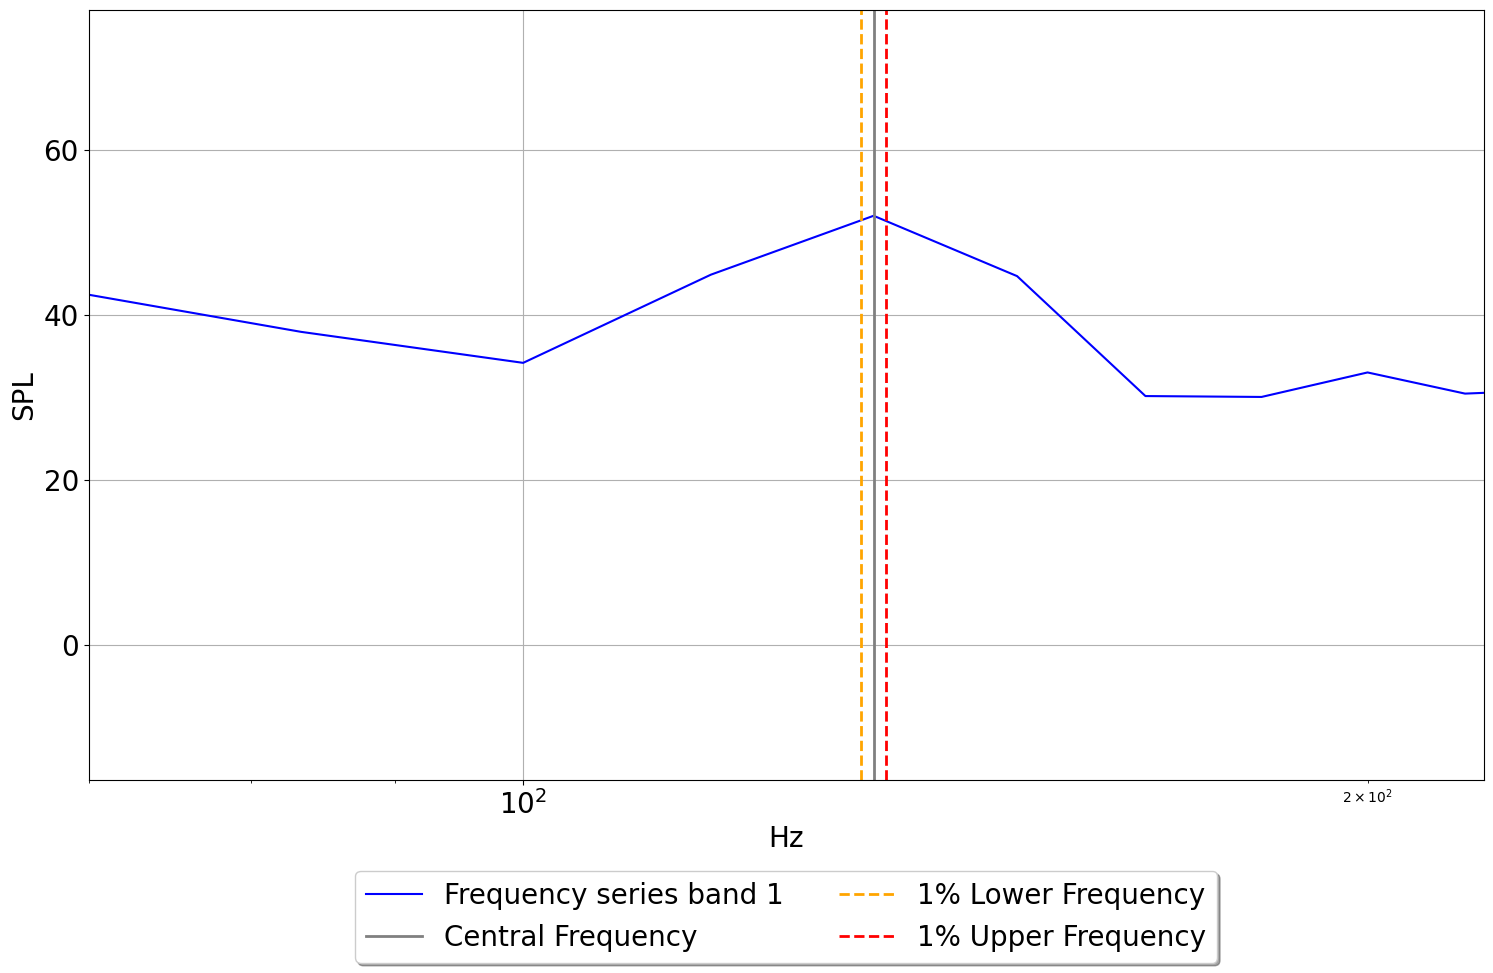
\includegraphics[width=0.70\linewidth]{Figures/spectra_band_1.png}
    \caption{1\% band}
    
\end{subfigure}%
\begin{subfigure}{.5\textwidth}
    \label{fig1b}
    \centering
    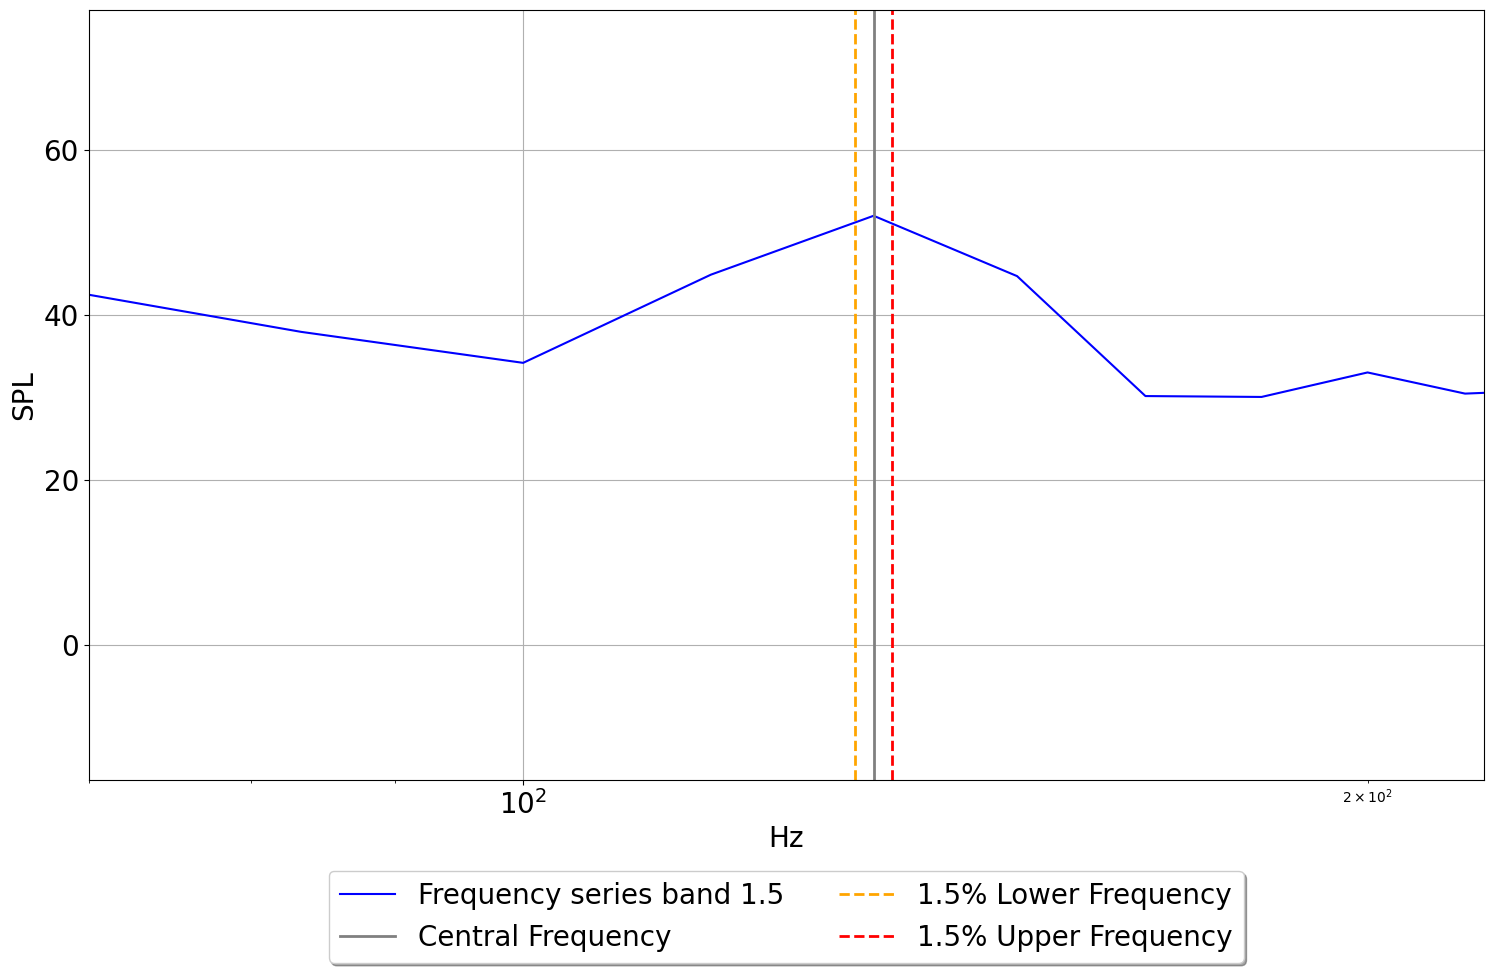
\includegraphics[width=0.70\linewidth]{Figures/spectra_band_1.5.png}
    \caption{1.5\% band}
    
\end{subfigure}
\begin{subfigure}{.5\textwidth}
    \label{fig1c}
    \centering
    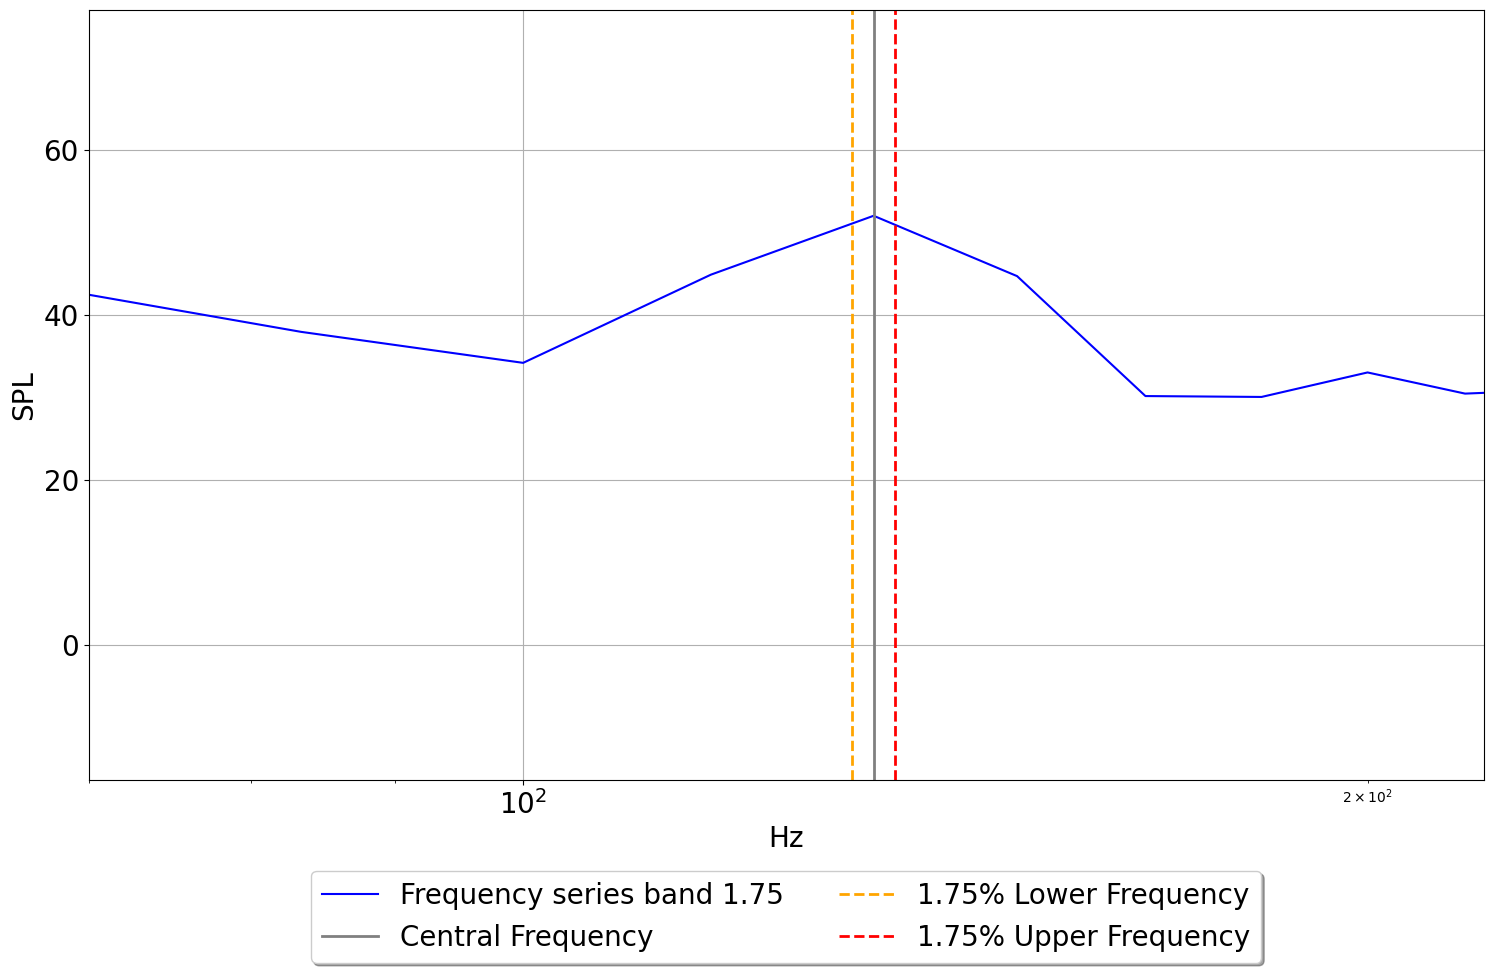
\includegraphics[width=0.70\linewidth]{Figures/spectra_band_1.75.png}
    \caption{1.75\%}
    
\end{subfigure}%
\begin{subfigure}{.5\textwidth}
    \label{fig1d}
    \centering
    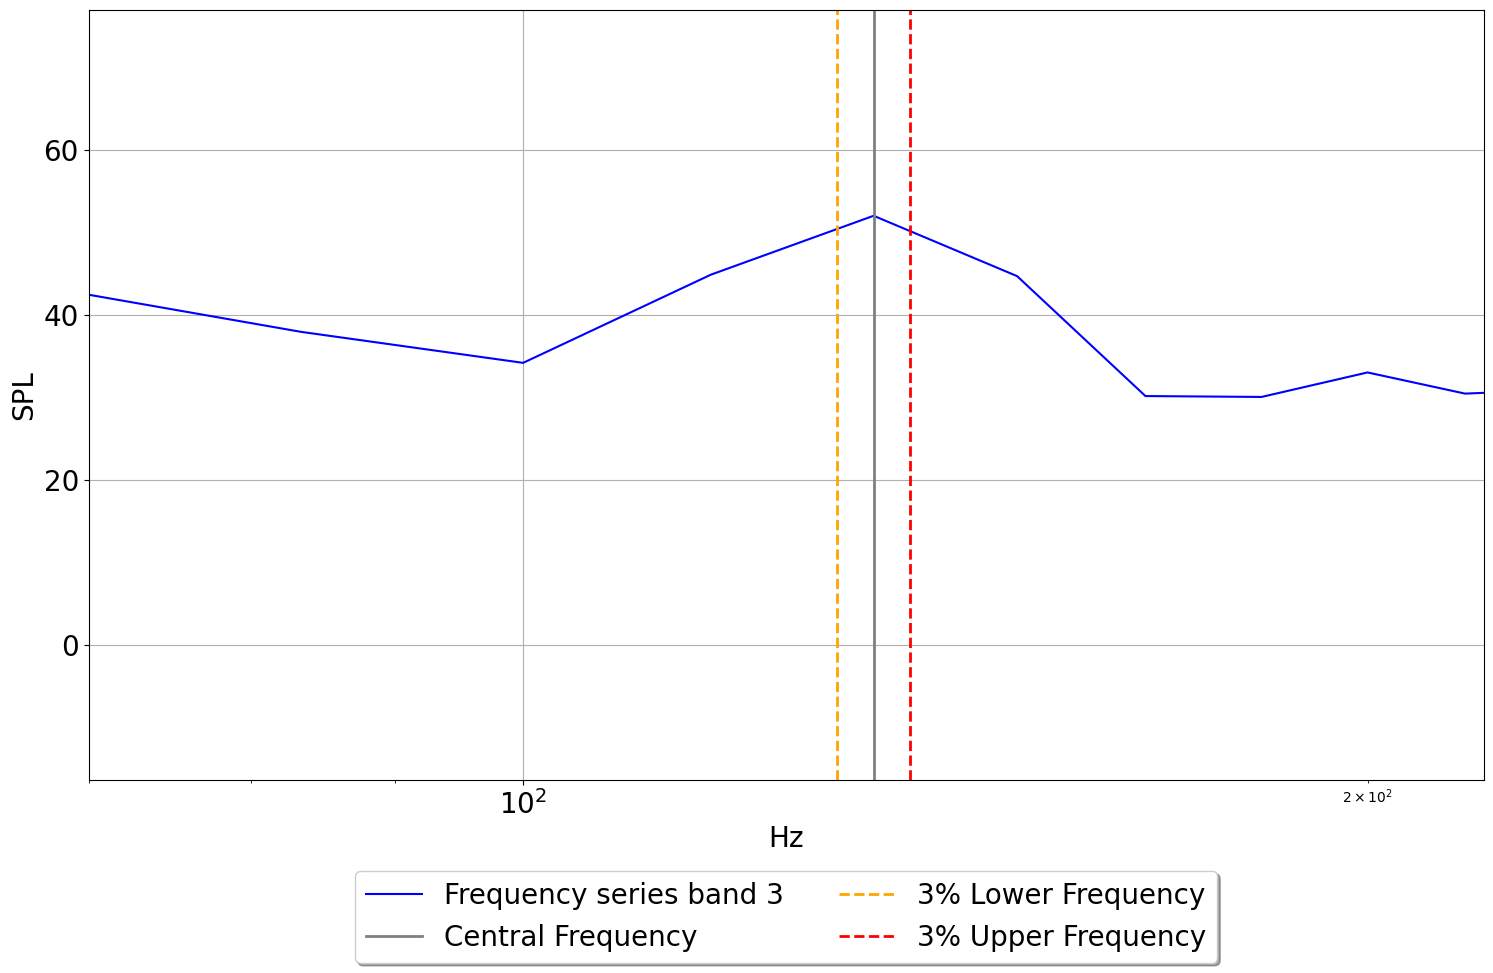
\includegraphics[width=0.70\linewidth]{Figures/spectra_band_3.png}
    \caption{3\% band}
    
\end{subfigure}%
\caption{Band analysis with diferent percentages}
\label{fig1}
\end{figure}
It is important to add that the band of interest choice is primarily empirical, which results in testing band percentages and assess the performance of the ones who fit the problem the most. In this study we manage to compare multiple band percentages with the experimental instantaneous rotational frequency of the propeller. 

Once the frequency band of the characteristic harmonic is selected, one may estimate the analytic signal according to \ref{eq2}, so that is possible to extract the analitical parameters of interest, such as the instantaneous phase of the propeller signal.


After the analytic signal is estimated, we shall extract the phase from one $\phi_{x} (t) = tan^{-1}(\hat{x}(t)/x(t))$. The phase is then normalized by dividing the phase by the order $m$ of the harmonic chosen in the first step. 
\begin{equation}
    \phi_{x,m} (t)=\frac{\phi_{x}(t)}{m} 
    \label{eq3}
\end{equation}

After this normalization, the angular position of the propeller in radians in determined. In order to facilitate later mathematical manipulations, the phase is transformed into a first degree function to ensure the proportionality of the angular signal obtained. This can be done easily with a Numpy build-in function.

The phase markers are defined to identify the moment where the propeller completes one rotation, which is when the index corresponds to $2\pi$ radians. This is achieved through a linear interpolation between time and phase. From these markers, it is possible to establish a list that records the complete rotations, thus allowing the rotation period to be determined.

Finally, the speed profile can be traced based on the propeller rotation period, since:
\begin{equation}
    f = \frac{1}{T} = \frac{1}{t_{i+1}-t_{i}}
    \label{eq4}
\end{equation}
Where the notation $t_{i}$ is the time instant $t$ where the phase marker $i$ is generated. 

\section{Synthetic, numerical and experimental setups}
In Sec. 2 was presented the demodulation techniques tested in this study to extract the instantaneous rotational frequencies of a propeller. The next step is to present the setups from which the data is created or extracted, so that is possible to test and check the feasibility of the method.

\subsection{Synthetic Signal}

\cite{bonomo} tested some decomposition techniques aimed in experimental propeller data, where it took account the rotational speed fluctuations. In this work, the same formulation is used and it is shown in 3 steps \citep{bonomo}:
\begin{enumerate}
    \item Generate a time array with the time-steps of $\Delta t >> 1/ fs$ where $fs$ is the desired sampling frequency for the synthetic signal.
    \item Generate a random instantaneous velocity array with the same lenght as the time array from step 1.
    \item Re-sample the velocity array from step 2 to have the same $fs$ as the desired synthetic signal. In this work, a cubic spline interpolation was used to provide a smooth curve. The resulting array  is the instantaneous frequency, $f_i(t)$ to be used in:
    \begin{equation}
        \label{eq5}
        \theta_i (t)=2\pi \int_{0}^{t}f_i (t)dt
    \end{equation}
\end{enumerate} 

Finally, the synthetic signal is the sum of modulated harmonic signals, which can be given by:
\begin{equation}
    \label{eq6}
    p(t) = \sum_{n=1}^{N} A_n sin(n\theta_i (t) + \phi_n) + w(t)
\end{equation}

Where N is the number of harmonics, $A_n$ is the harmonic amplitude, $\theta_i$ is the instantaneous phase angle defined in \ref{eq5}, $\phi_n$ is a random phase angle with a uniform distribution in the interval $[0,2\pi]$ and $w(t)$ is a Gaussian white noise that represents the broadband component of the propeller signal.

\subsection{Experimental setup}
The UFSC Isolated Propeller Test Rig is installed in the semi-anechoic chamber at the Laboratory of Vibration and Acoustics (LVA/UFSC) \citep{Augusto}. The propeller rig structure primarily consists of an aluminum frame mounted on a steel column bolted to the ground. A brushless DC motor, specifically the U3 KV700 model from T-Motor, is utilized to drive
motion to the propellers, in conjunction with an Electronic Speed Controller (ESC), the ALPHA 40A, also from T-Motor.
Rotational speed and angular position monitoring are facilitated by a digital laser indexed encoder, the EM1 from US
Digital, with 50 cycles per revolution (CPR).
The rotational speed of the propeller is controlled via an in-house closed-loop PID controller, implemented in
Python3, utilizing a PXIe-6368 Multi-function DAQ as a hardware interface. The controller operates with an average
update rate of 30 Hz.

An array of microphones, oriented towards the ground, is positioned in line at a distance of 1.6 m from the steel column, parallel and 2 m away from the propeller axis. The array is arranged to cover a range from -45° to 45°, with 0° representing the rotor disk plane and positive angles measured above the rotation plane. Comprising nine GRAS 46AE 1/2” free-field microphones, the array includespositions at angular offsets of -27.5°, 0° and 27.5°, numbered 3, 5 and 7, respectively. The minimum ratio of the distance between microphones and the hub r to the propeller diameter d was r/d = 6.5, ensuring all microphones were positioned in the acoustic far field. The microphone array is presented in Fig.2.
\begin{figure}[h!]
    \centering
    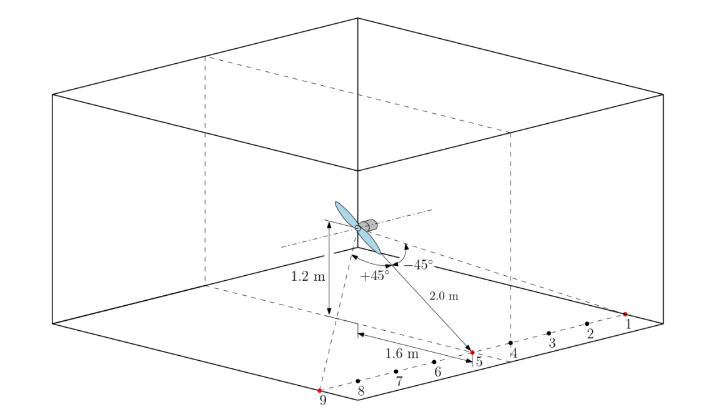
\includegraphics[angle=0, scale=0.320]{Figures/ufsc_microphone_array.png}
    \caption{UFSC test rig microphone array displacement}
    \label{fig2}
    \end{figure}

All signals are simultaneously acquired using custom software implemented in Python3, utilizing the nidaqmx
library. The signals are acquired with PXIe-4499 modules by National Instruments, with a sampling frequency of 51.2 kHz during 30 s runs for each test condition. \citep{Augusto}. The overview of the propeller mounted is shown in Fig.3.
\begin{figure}[h!]
    \centering
    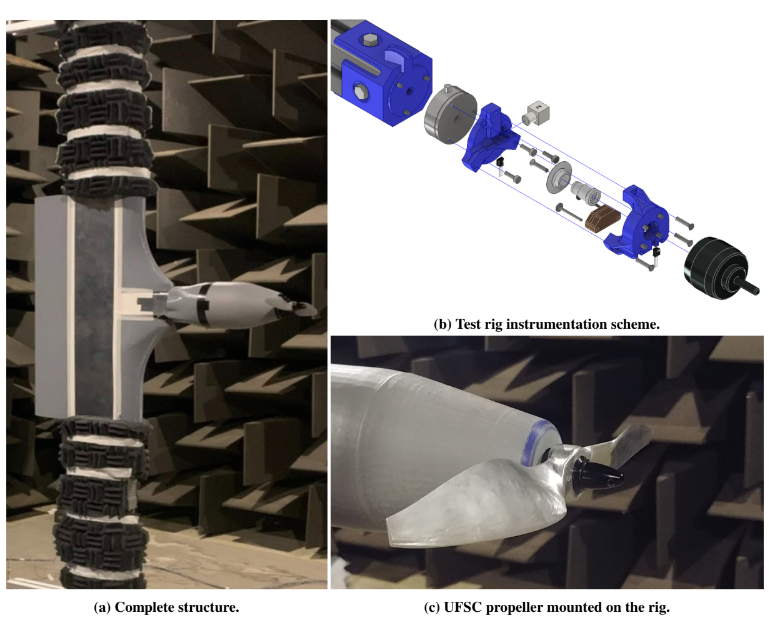
\includegraphics[angle=0, scale=0.320]{Figures/UFSC_propeller_test_rig.png}
    \caption{UFSC propeller test rig}
    \label{fig3}
    \end{figure}
\section{Results}
\subsection{Synthetic signal}
\subsection{Experimental signal}
Regarding the selection of the propeller signal frequency band, as mentioned in Section 2, the characteristic frequency of the harmonic given by the first BPF was chosen as the central frequency, characterized as the tone with the highest energy. The frequency band variation was 0.1\%, 0.5\%, 0.75\%, 1\%, 1.2\%, 1.5\%, 1.75\%, 2\%, and 3\% of this frequency, both above and below.

Below 0.1\%, it was observed that the instantaneous frequency variation was cut off due to the narrow band in the spectrum, and above 3\%, the result began to diverge due to the excessively wide band in the characteristic tone.


\section{Conclusion}


\bibliographystyle{abcm}
\renewcommand{\refname}{}
\bibliography{bibfile}

\section{RESPONSIBILITY NOTICE}

The following text, properly adapted to the number of authors, must be included in the last section of the paper:

The author(s) is (are) solely responsible for the printed material included in this paper.

\end{document}
